%%%%%%%%%%%%%%%%%%%%%%%%%%%%%%%%%%%%%%%%%%%%%%%%%%%%%%%%%%%%%%
%% Carlos Segarra's Beamer Presentation Template. All credits
%% to Vincent Labatut from whom I took the template and added
%% my own flavour to it. Kudos to <vincent.labatut@univ-avignon.fr>
%%%%%%%%%%%%%%%%%%%%%%%%%%%%%%%%%%%%%%%%%%%%%%%%%%%%%%%%%%%%%%
% setup Beamer
\documentclass[10pt,    % default is 11pt, use 10pt for more compact slides
%    handout,            % collapse all overlays (=animations) and video-invert console text
    english,            % presentation language (theme supports only french & english)
    xcolor=table,       % colors in the tables
    envcountsect,        % include section number in theorem numbers
    aspectratio=169     % Using 16:9 aspect ratio because 2019
]{beamer}

%%%%%%%%%%%%%%%%%%%%%%%%%%%%%%%%%%%%%%%%%%%%%%%%%%%%%%%%%%%%%%
% setup the theme
%\usepackage{au/sty/beamerthemeAU}         % no option at all
\usepackage[light]{csg-temp/sty/beamerthemeAU}   % the "light" option only changes the title and section pages

%%%%%%%%%%%%%%%%%%%%%%%%%%%%%%%%%%%%%%%%%%%%%%%%%%%%%%%%%%%%%%
% setup side notes
\usepackage{pgfpages}                                   % comment all 3 below lines to hide notes
%\setbeameroption{show notes}                           % alternate content and note slides
%\setbeameroption{show only notes}                      % only note slides
%\setbeameroption{show notes on second screen=right}    % dualscreen: right, left, top, bottom
%\usepackage{enumitem}

%%%%%%%%%%%%%%%%%%%%%%%%%%%%%%%%%%%%%%%%%%%%%%%%%%%%%%%%%%%%%%
% name of the biblatex file
\addbibresource{biblio.bib}

%%%%%%%%%%%%%%%%%%%%%%%%%%%%%%%%%%%%%%%%%%%%%%%%%%%%%%%%%%%%%%
% External Packages
\usepackage{datenumber}
\usepackage{varwidth}

% Math Mode
%\usepackage{algorithm}
%\usepackage{algorithmic}
%\usepackage{algorithm2e}
%\usepackage{multicol}
%\usepackage[noend]{algpseudocode}

%%%%%%%%%%%%%%%%%%%%%%%%%%%%%%%%%%%%%%%%%%%%%%%%%%%%%%%%%%%%%%
% title and subtitle of the presentation (the latter is optional)
\subtitle{Decentralized Systems} % leave empty if no subtitle
\title[Decentralized Systems] % leave empty for no title in footer
    {\normalsize Bittorrent Traffic Optimization \\ \Large Bittorrent traffic optimization in \\ \Large Wireless Mesh Networks with ALTO Service }
\subtitle{Master in Research in Informatics - MIRI}
%%%%%%%%%%%%%%%%%%%%%%%%%%%%%%%%%%%%%%%%%%%%%%%%%%%%%%%%%%%%%%
% date of the presentation (leave empty for no date, default is today)
\date[March 3, 2020] % leave empty for no date in footer
    {Tuesday March 3, 2020}
    %{\datedayname, \today}
%%%%%%%%%%%%%%%%%%%%%%%%%%%%%%%%%%%%%%%%%%%%%%%%%%%%%%%%%%%%%%
% authors and their affiliations (the latter is optional)
\author[] % leave empty for no author in footer
{F. Paolo d'Elia, G. Di Stasi, S. Avallone, R. Canonico \\\small \textit{Presented by} Carlos Segarra - \texttt{carlos.segarra@estudiant.upc.edu}}
%{\inst{1} Computer Science Lab, Avignon University -- LIA EA 4128 \texttt{\{firstname.lastname\}@univ-avignon.fr}
%\and \inst{2} Institute of Disruptive Innovation, University of Excellence \texttt{\{firstname.lastname\}@univ-excell.fr}
%}
%%%%%%%%%%%%%%%%%%%%%%%%%%%%%%%%%%%%%%%%%%%%%%%%%%%%%%%%%%%%%%
% optional: additional logo (ex. lab)
%\titlegraphic{
\includegraphics[width=3cm,]{images/logo_FME.png}}
% if you want several logos, put them in a box
%\titlegraphic{\parbox{3cm}{\includegraphics[width=3cm,]{images/ceri_logo.pdf}\newline\includegraphics[width=3cm,]{images/lia_logo.pdf}}}
%%%%%%%%%%%%%%%%%%%%%%%%%%%%%%%%%%%%%%%%%%%%%%%%%%%%%%%%%%%%%%

%%%%%%%%%%%%%%%%%%%%%%%%%%%%%%%%%%%%%%%%%%%%%%%%%%%%%%%%%%%%%
% Presentation speciphic packages
% \usepackage{multicol}
% \usepackage[titles]{tocloft}
% \renewcommand{\cftchapfont}{\normalfont\bfseries}
\usetikzlibrary{decorations.pathmorphing, patterns}
\usepackage{tabularx}
\newcolumntype{L}[1]{>{\raggedright\arraybackslash}p{#1}}
\newcolumntype{C}[1]{>{\centering\arraybackslash}p{#1}}
\newcolumntype{R}[1]{>{\raggedleft\arraybackslash}p{#1}}
%%%%%%%%%%%%%%%%%%%%%%%%%%%%%%%%%%%%%%%%%%%%%%%%%%%%%%%%%%%%%

%%%%%%%%%%%%%%%%%%%%%%%%%%%%%%%%%%%%%%%%%%%%%%%%%%%%%%%%%%%%%%
\begin{document}
%%% title page
\begin{frame}
  \titlepage
\end{frame}

\begin{frame}
    \frametitle{General Information}

    \begin{itemize}
        \item \textbf{Full Title:} "Bittorrent traffic optimization in Wireless Mesh Networks with ALTO service" $[1]$
        \item \textbf{Authors:} Francesco Paolo d'Elia, Giovanni Di Stasi, Stefano Avallone, and Roberto Canonico
        \item \textbf{Published At:} \href{https://ieeexplore.ieee.org/xpl/conhome/5976314/proceeding}{2011 IEEE International Symposium on a World of Wireless, Mobile and Multimedia Networks}
        \item \textbf{Publishing Date:} 20-24 June 2011
        \item \textbf{DOI:} \href{https://doi.org/10.1109/WoWMoM.2011.5986177}{10.1109/WoWMoM.2011.5986177}
    \end{itemize}


    \small
    \begin{description}
        \item $[1]$ F. P. D'Elia, G. Di Stasi, S. Avallone and R. Canonico, "Bittorrent traffic optimization in Wireless Mesh Networks with ALTO service," 2011 IEEE International Symposium on a World of Wireless, Mobile and Multimedia Networks, Lucca, 2011, pp. 1-6
    \end{description}
 

\end{frame}

\begin{frame}
    \frametitle{TL-DR}
    \framesubtitle{A Ten Thousand Feet View}

    \vspace{-25pt}

    \begin{alertblock}{Main Contribution}
        The paper presents a \textbf{hierarchichal peer organization} to optimize Bittorrent's bandwidth usage in wireless mesh networks.
    \end{alertblock}

    \begin{block}{Techniques}
        The authors base on the \textbf{Application Layer Traffic Optimization Service} which provides the peers with knowledge about the underlying network.
    \end{block}

    \begin{alertblock}{Evaluation Results}
        They report a $27\%$ time reduction in \textbf{download time} and a $66\%$ inter-region \textbf{traffic} reduction.
    \end{alertblock}

\end{frame}

\begin{frame}
    \frametitle{Background Concepts}
    \framesubtitle{Bittorrent \& ALTO}

    \begin{columns}
        \begin{column}{.55\textwidth}
            \textbf{Tracker-Based Bittorrent Protocol:}
            \begin{itemize}
                \item \textbf{Bittorrent} is a peer-to-peer communication protocol for file sharing.
                \item A \textbf{Bittorrent} tracker is a server that assists in the communication between peers.
                \item It keeps track of where file copies reside.
            \end{itemize}
            \textbf{The ALTO Service Architecture:}
            \begin{itemize}
                \item The \textbf{\href{https://tools.ietf.org/html/rfc7285}{Application Layer Traffic Optimization}} services provide network information with the goal of modifying network resources consumption.
            \end{itemize}
        \end{column}
        \hfill
        \begin{column}{.35\textwidth}
            \begin{figure}[h!]
                \centering
                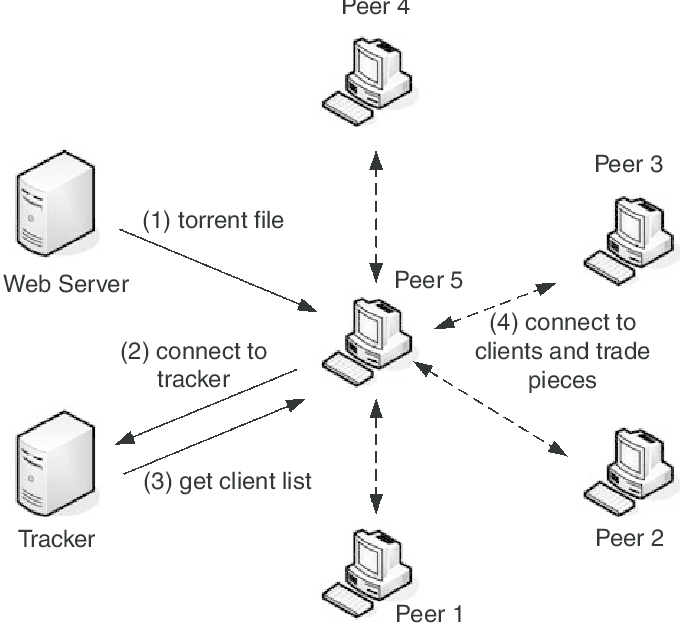
\includegraphics[width=\textwidth]{./images/bit-torrent.png}
                \caption{Bittorrent Tracker Protocol Architecture}
            \end{figure}
        \end{column}
    \end{columns}

\end{frame}

\begin{frame}
    \frametitle{Proposed Architecture}

    \vspace{-15pt}
    \begin{columns}
        \begin{column}{.35\textwidth}
            \textbf{Exectuion Flow:}
            \begin{enumerate}
                \item Peer node queries tracker for list of peers.
                \item Tracker forwards request to ALTO Server.
                \item Server delegates to respective WMN Agent.
                \item Server aggregates responses and returns sorted list to Tracker.
                \item Tracker forwards response to asking peer.
            \end{enumerate}
        \end{column}
        \begin{column}{.70\textwidth}
            \begin{figure}[h!]
                \centering
                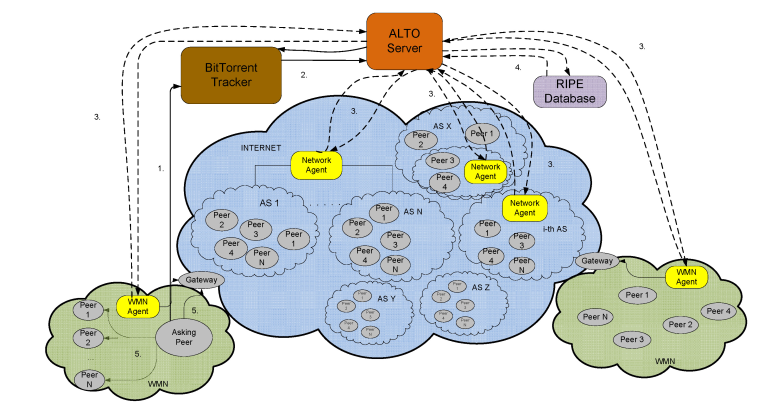
\includegraphics[width=1.05\textwidth]{./images/architecture.png}
            \end{figure}
        \end{column}
    \end{columns}

\end{frame}

\begin{frame}
    \frametitle{Open Questions}

    \begin{enumerate}
        \item What's your opinion about the evaluation section?
        \begin{itemize}
            \item What experiments do they lay out?
            \item What do they show?
            \item What does that prove?
            \item What is the statistical relevance of the results?
            \item Who they compare against?
        \end{itemize}
        \item Are Tracker-Based Bittorent Protocols used anymore?
        \item What's your opinion on the design choice for the ALTO Server?
    \end{enumerate}

\end{frame}



\end{document}
